\section*{MPI Implementation}
The second parallel implementation utilizes the \texttt{OpenMPI} and \texttt{OpenMP} \texttt{C++} libraries. \texttt{OpenMPI} is an open-source implementation of the \texttt{MPI} standard, which provides a message-passing interface to enable communication between multiple processes, often distributed across different nodes in a cluster or supercomputer. \texttt{OpenMP}, similar to \texttt{FastFlow}, simplifies parallel programming within shared-memory systems by enabling efficient use of multiple processors or cores within a single node.

\par In this version of the algorithm, \texttt{OpenMPI} handles communication between nodes, while \texttt{OpenMP} is employed inside each node to parallelize local computation. In contrast to the previous implementation, this solution operates in a distributed memory environment, where each node functions as an independent process with its own local memory. As a result, explicit communication between nodes is necessary to share data and coordinate tasks.

\subsection*{The Divide et Impera approach}

\par To optimize the balance between local computation and inter-process communication, a \textit{Divide et Impera} strategy has been employed. At the start of execution, the system consists of $n$ nodes, each of which can assume the role of either \texttt{Master} or \texttt{Supporter}. A \texttt{Master} can have up to two \texttt{Supporter}s, while each \texttt{Supporter} is associated with only one \texttt{Master}. \texttt{Master}s do not share \texttt{Supporter}s with one another.

After determining their roles and associations independently, each node computes a submatrix of the final matrix. The size of each submatrix is determined by dividing the entire matrix by the number of active processes, while the portion of elements is determined by an id associated to the node. Once a \texttt{Supporter} has completed its assigned submatrix, it sends the result to its \texttt{Master}. The \texttt{Master} then merges the received results with its own computation.

After merging, the \texttt{Supporter}s terminate their execution, decreasing the number of active processes. The remaining \texttt{Master}s redetermine their roles, potentially becoming \texttt{Supporter}s, and the process iterates. The algorithm concludes when only one node remains, referred to as the \texttt{Last} node, which computes the final portion of the matrix and completes the execution. A pseudocode describing a node behaviour of this approach is shown in Algorithm \ref{Algo3}.

\begin{algorithm}
\begin{algorithmic}
\WHILE{TRUE}
    \STATE role = DetermineMyRole();
    \STATE ComputeMySubMatrix();
    \IF{I am a Master or a Supporter}
        \STATE MergeMatrices();
    \ENDIF
    \IF{I am a Supporter or the Last active node}
        \STATE EndExecution();
    \ENDIF
\ENDWHILE
\end{algorithmic}
\caption{Wavefront Pattern for a node in the MPI algorithm}
\label{Algo3}
\end{algorithm}


\begin{figure}[h]
    \centering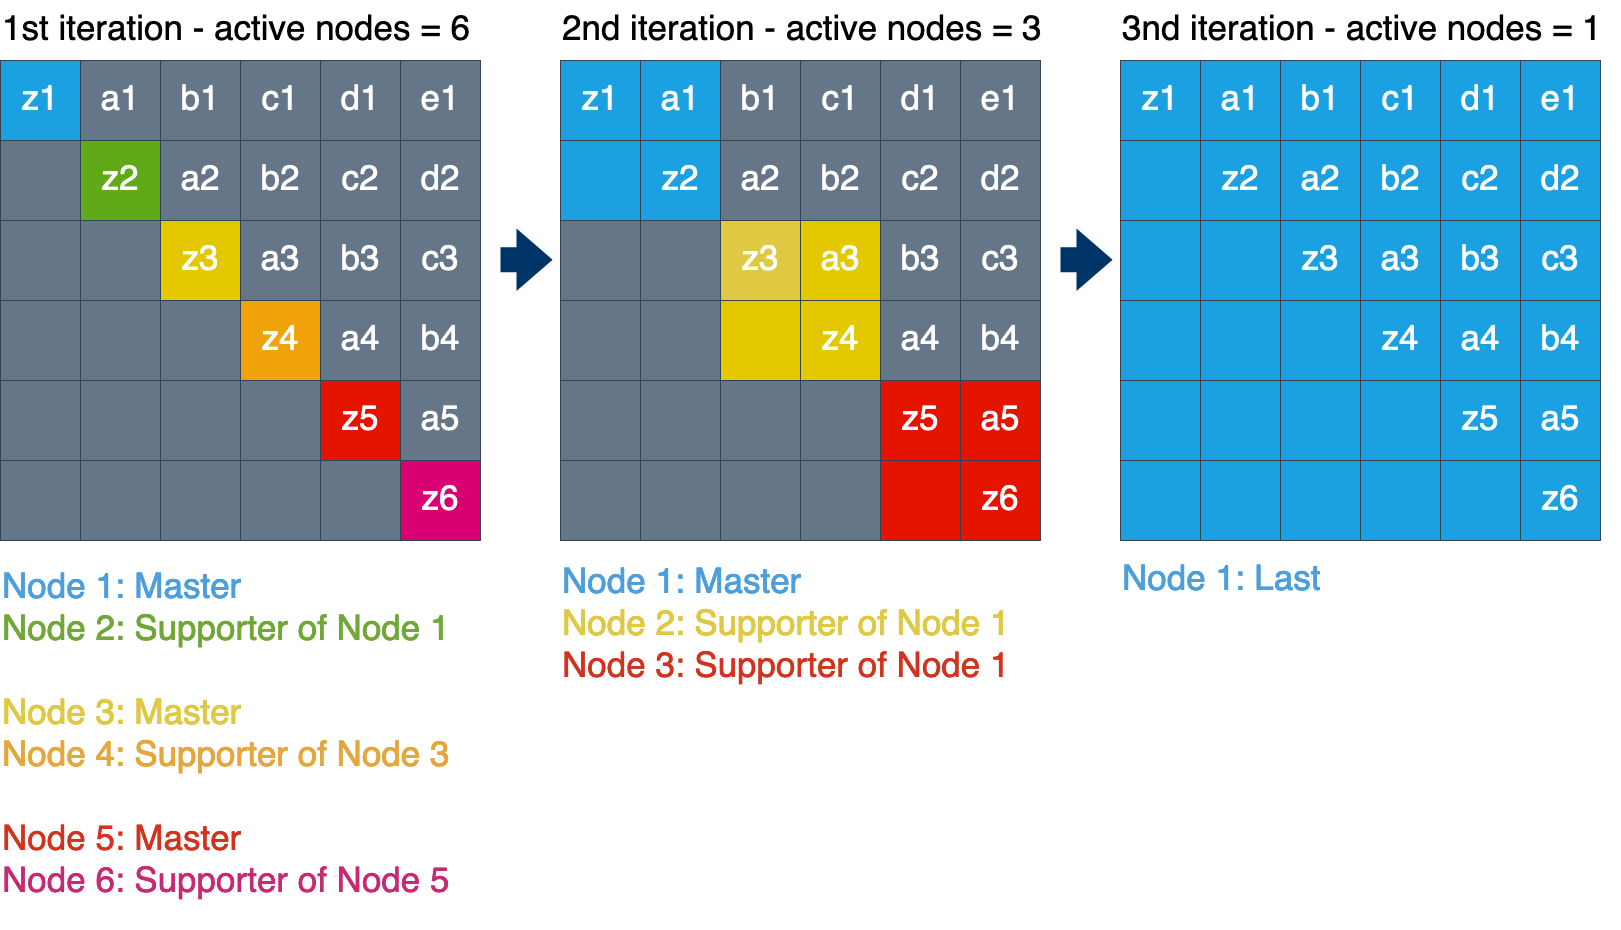
\includegraphics[scale=0.30]{img/MPI/DivideEtImpera.drawio.png}
    
    \caption{Example of an execution of the MPI parallel algorithm}
\end{figure}


\subsection*{OpenMP usage}
\texttt{OpenMP} is utilized within a node to compute its submatrix. Previous implementations have shown that both the computation of elements along the same diagonal and the dot product computation for individual elements can be parallelized. Both parallelization are achieved using separate \texttt{Parallel For} constructs. In the case of the dot product computation, since the local multiplications needs to be summed to obtain the final result, the \texttt{reduction} paradigm is employed to combine these local copies into a final value. Additionally, \texttt{OpenMP} is used by both roles when merging their matrices. Because the rows to be copied are distinct, these communications can be executed concurrently.

\subsection*{Determining the role of a Node}
As previously mentioned, a node can take on one of three roles: \texttt{Master}, \texttt{Supporter}, or \texttt{Last}. The role of a node is determined at the beginning of each iteration based on its \texttt{id}, the number of active nodes, and the size of the final matrix. If the matrix size is smaller than the number of nodes, the excess nodes are removed at the start of the computation as they are not needed. The node's \texttt{id} is recalculated at each iteration: initially, it matches the \texttt{rank} assigned by \texttt{MPI}, but in subsequent iterations, it depends on the number of active nodes. \texttt{id}s begin at zero. The relation between the \texttt{rank} of a node and its \texttt{id} is the following:

\begin{equation}
    current\_id = \lceil rank / 2^{current\_iteration - 1}\rceil
\end{equation}

A \texttt{Master} node is always assigned an even \texttt{id} and must have an adjacent node. \texttt{Supporter} nodes either have an odd \texttt{id} or are even-numbered without any following nodes. Once a \texttt{Supporter} node completes its computation, it exits the Wavefront computation and waits for the program to terminate. Thus the number of active nodes at each iteration is equal to the previous one divided by two. The \texttt{Last} node is, as the name implies, the only node left in the final iteration. It has a unique role since it is the only node that does not need to merge its matrix with any other node; it computes the remaining elements and then exits the computation.

\subsection*{Communication between nodes}
After completing the computation of its sub-matrix, a node must exchange data with its partners, either sending its own results or receiving results from others. A node can communicate only with its associated \texttt{Master} or \texttt{Supporter}s. During the role determination of a node, the algorithm also identify the \texttt{rank}s of the nodes it needs to communicate with. For a \texttt{Supporter}, the node stores the rank of the \texttt{Master} in the variable \texttt{my\_master}, while for a \texttt{Master}, it stores the \texttt{rank}s of its \texttt{Supporter}s in the vector \texttt{my\_supporters}. The \texttt{MergeMatrices} method manages this communication.

\par In this method, both roles determine which rows to send or receive based on the final matrix configuration. The rows are calculated using the \texttt{Supporter} node's \texttt{id} as follows:

\begin{align*}
    first\_row &= supporter\_id \times sub\_mtx\_length \\
    last\_row &= first\_row + (sub\_mtx\_length - 1) \\
    num\_rows &= (last\_row - first\_row) + 1
\end{align*}

Next, the process identifies for each row, regarding its role, the index of the first element computed by the \texttt{Supporter}. Communication is then handled synchronously using either \texttt{MPI\_Send} or \texttt{MPI\_Recv}, depending on the role. The \texttt{std::vector<double>} containing the data is passed as a buffer, offset to the calculated index, and $lenght\_sub\_matrix$ elements are retrieved. Since each send/receive is done on a different row, the process is sped up through parallelization using the \texttt{Parallel For} construct.

This implementation still exploits the locality of reference principle storing a copy of the columns of the upper-triangular as rows of the lower-triangular part, thus these values are considered during the copy. Although it might seem beneficial to send only the necessary elements of a row, rather than copying repeating elements, this avoids the \texttt{Master} to copy manually the received elements in their transposed position on the lower-triangular matrix. 

\begin{figure}[h]
    \centering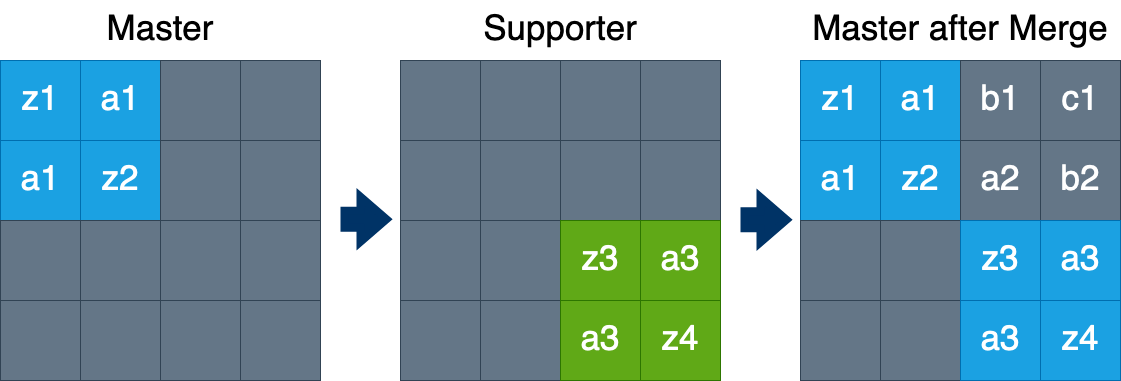
\includegraphics[scale=0.25]{img/MPI/MergeMatrix.drawio.png}
    
    \caption{Example of merging the matrices of a Master and its associated Supporter.}
\end{figure}

\subsection*{The WavefrontNode Class}
Each process spawned by \texttt{MPI} creates an instance of the \texttt{WavefrontNode} class. This class encapsulates all the methods and variables required for a node to perform the necessary computations. Upon creation, the constructor initializes essential information such as the node's \texttt{id} and \texttt{rank}, and then calls the \texttt{WaveFrontComputation()} method, which implements the pseudocode outlined in Algorithm \ref{Algo3}. By the end of the program, the node assigned the role of \texttt{Last} holds the final matrix, which is stored as a \texttt{SquareMatrix} object within itself.

\subsection*{Asymptotic Complexity}
Compared to the \texttt{FastFlow} algorithm, the asymptotic complexity of the current solution is theoretically more efficient. This is because each node computes a smaller portion of the overall matrix, and during the computation it can leverage both diagonal and dot product parallelism. Assuming the communication cost for sending/receiving  a single element of the matrix is $\mathcal{O}(1)$, and the cost for determining the node's current role is also $\mathcal{O}(1)$, then:
\begin{itemize}


    \item \textbf{Complexity of computing a single sub matrix =} $\mathcal{O}(\max{sub\_matrix\_length}) = \mathcal{O}((n-1)/ num\_nodes )$ where $n$ is the length of the matrix and $num\_nodes$ is the number of nodes employed in the pattern.

    \item \textbf{Complexity of sending/receiving a single row =} $row\_length \times \mathcal{O}(1) = \mathcal{O}(row\_length) = \mathcal{O}(n - 1)$ where $n$ is the length of the matrix

    \item \textbf{Complexity of merging matrices =} $2 \times \mathcal{O}(row\_length) = \mathcal{O}(n - 1)$

    \item \textbf{Complexity of an iteration for one node =} $ \mathcal{O}(1) + \mathcal{O}(n - 1) + \mathcal{O}((n-1)/ num\_nodes) = \mathcal{O}(n-1)$

    \item \textbf{Overall Complexity =} $ \sum_{iteration = 0}^{(n-1) / num\_nodes}{\mathcal{O}(n-1)} = \mathcal{O}(n-1)^{2}$
\end{itemize}

However, as the measurement section will demonstrate, approximating the communication is overly optimistic. In reality, for smaller matrices, the communication overhead significantly impacts the overall complexity, making it less efficient than the previous shared memory solution and in some cases even the sequential case.

\subsection*{Measurements}
The C++ implementation can be found in \texttt{src\_parallel\_mpi.cpp}. It's important to note that the program must be executed using the command \texttt{mpirun -N [number of nodes]}; otherwise, it will run sequentially. The implementation has been thoroughly tested with various matrix sizes and different numbers of nodes. Additionally, the behavior of the program has been evaluated both when dedicating an entire cluster node to a single program node and when assigning multiple program nodes to each machine in the cluster. Interestingly, assigning more than one process per node results in worse performance compared to the standard case as Figure \ref{MPI_THEADS} shows. This likely occurs because, although each process handles smaller matrices and the initial \texttt{Master-Supporter} pairs are typically assigned to processes within the same machine, resulting in lower communication overhead compared to contacting processes on different nodes, the increased overhead of managing more processes still outweighs these benefits.

\par For relatively small matrices (up to 1024 in length), the execution is slower than previous approaches due to communication overhead. Our tests showed minimal optimization when increasing the number of nodes from four to eight. As illustrated in Figure \ref{MPI_Speedup}, even though each node handles smaller matrices, the communication overhead of managing additional nodes negates any potential gains. Overall, in the matrices we tested, the \texttt{FastFlow} implementation outperforms \texttt{MPI}, obviously, as accessing the matrix within a shared memory environment is significantly faster than passing submatrices.

\begin{figure}[h!]
    \centering
    % First row: Two images adjacent
    \begin{minipage}[t]{0.49\textwidth}
        \centering
         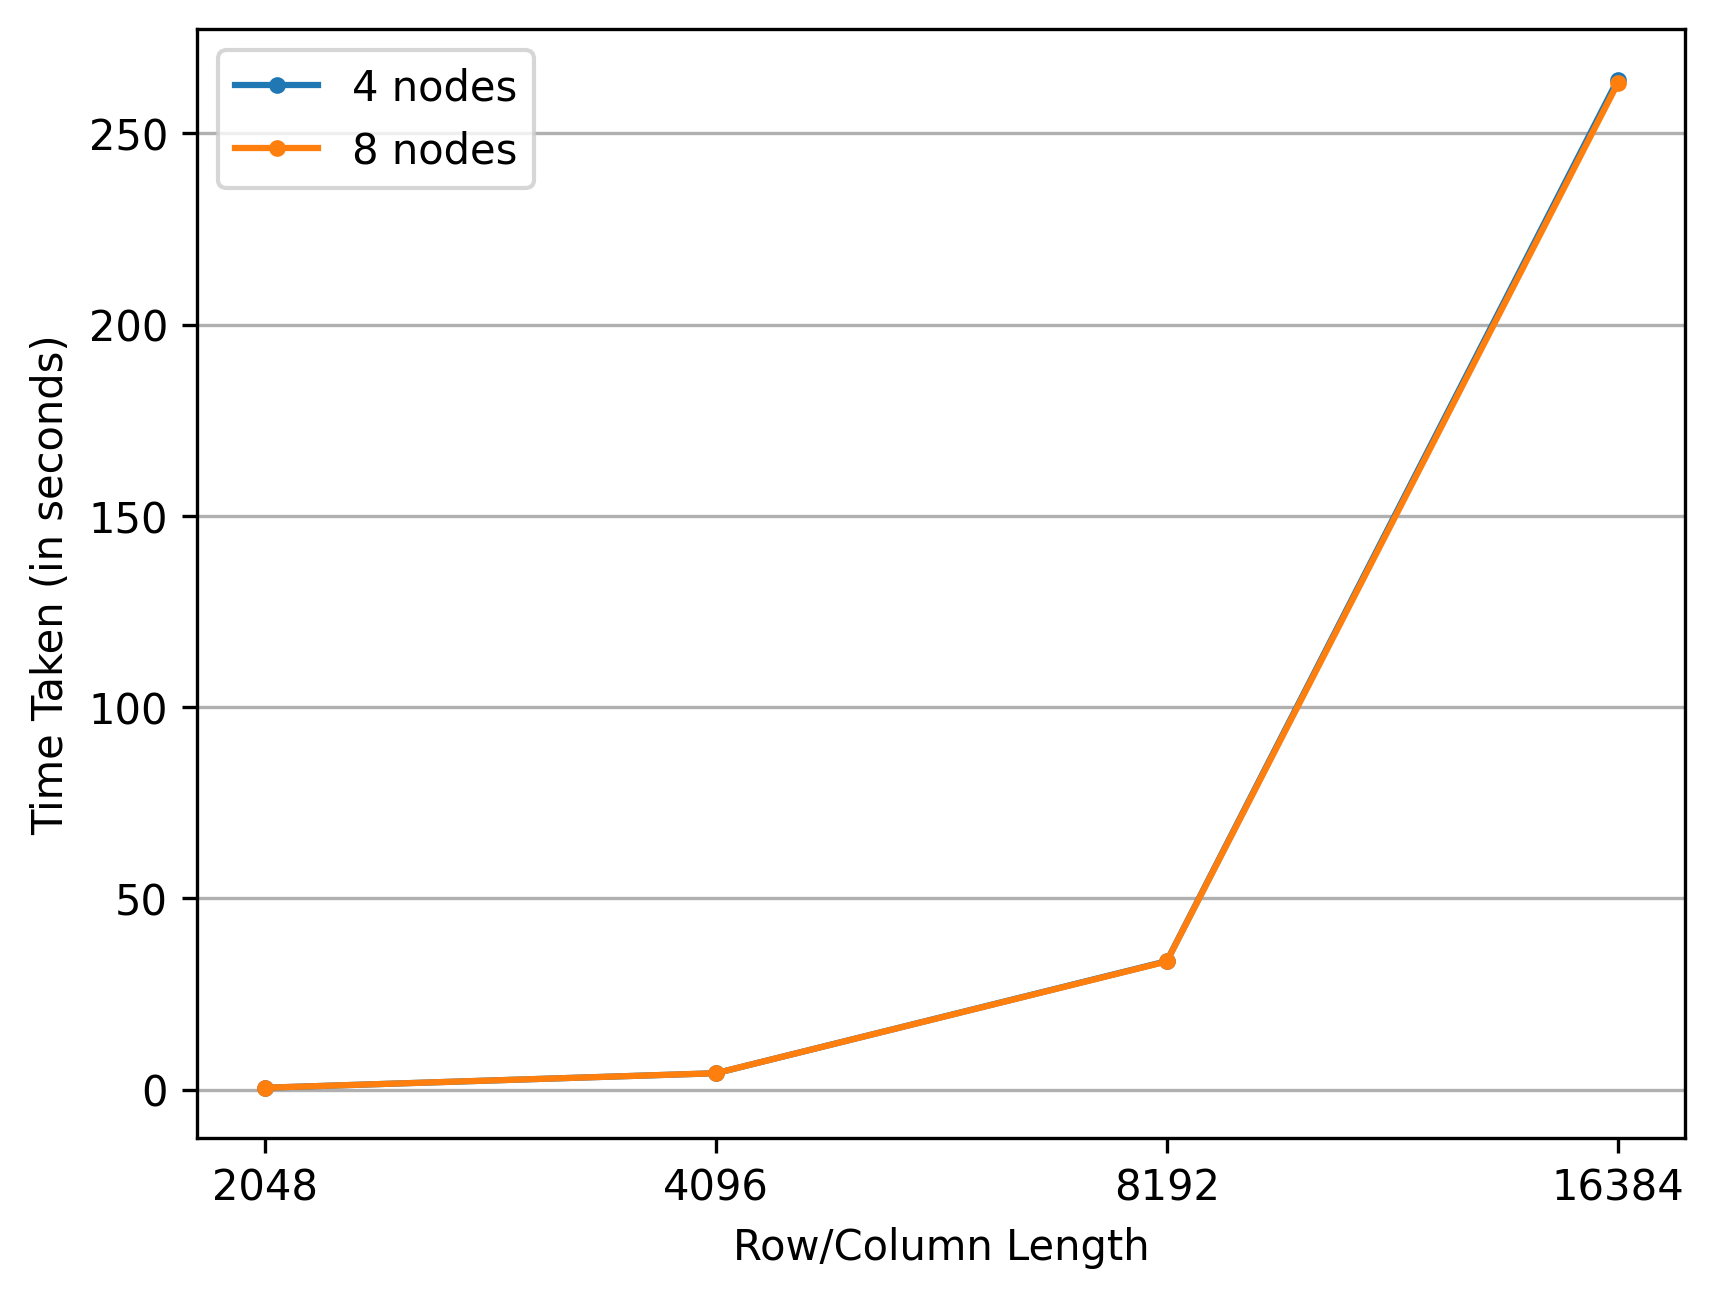
\includegraphics[width=\textwidth]{img/MPI/mpi_strong_scaling.png}
        \caption{Comparison between MPI using 4 or 8 nodes}
        \label{MPI_4_8_NODES}
    \end{minipage}
    \hfill
    \begin{minipage}[t]{0.49\textwidth}
        \centering
        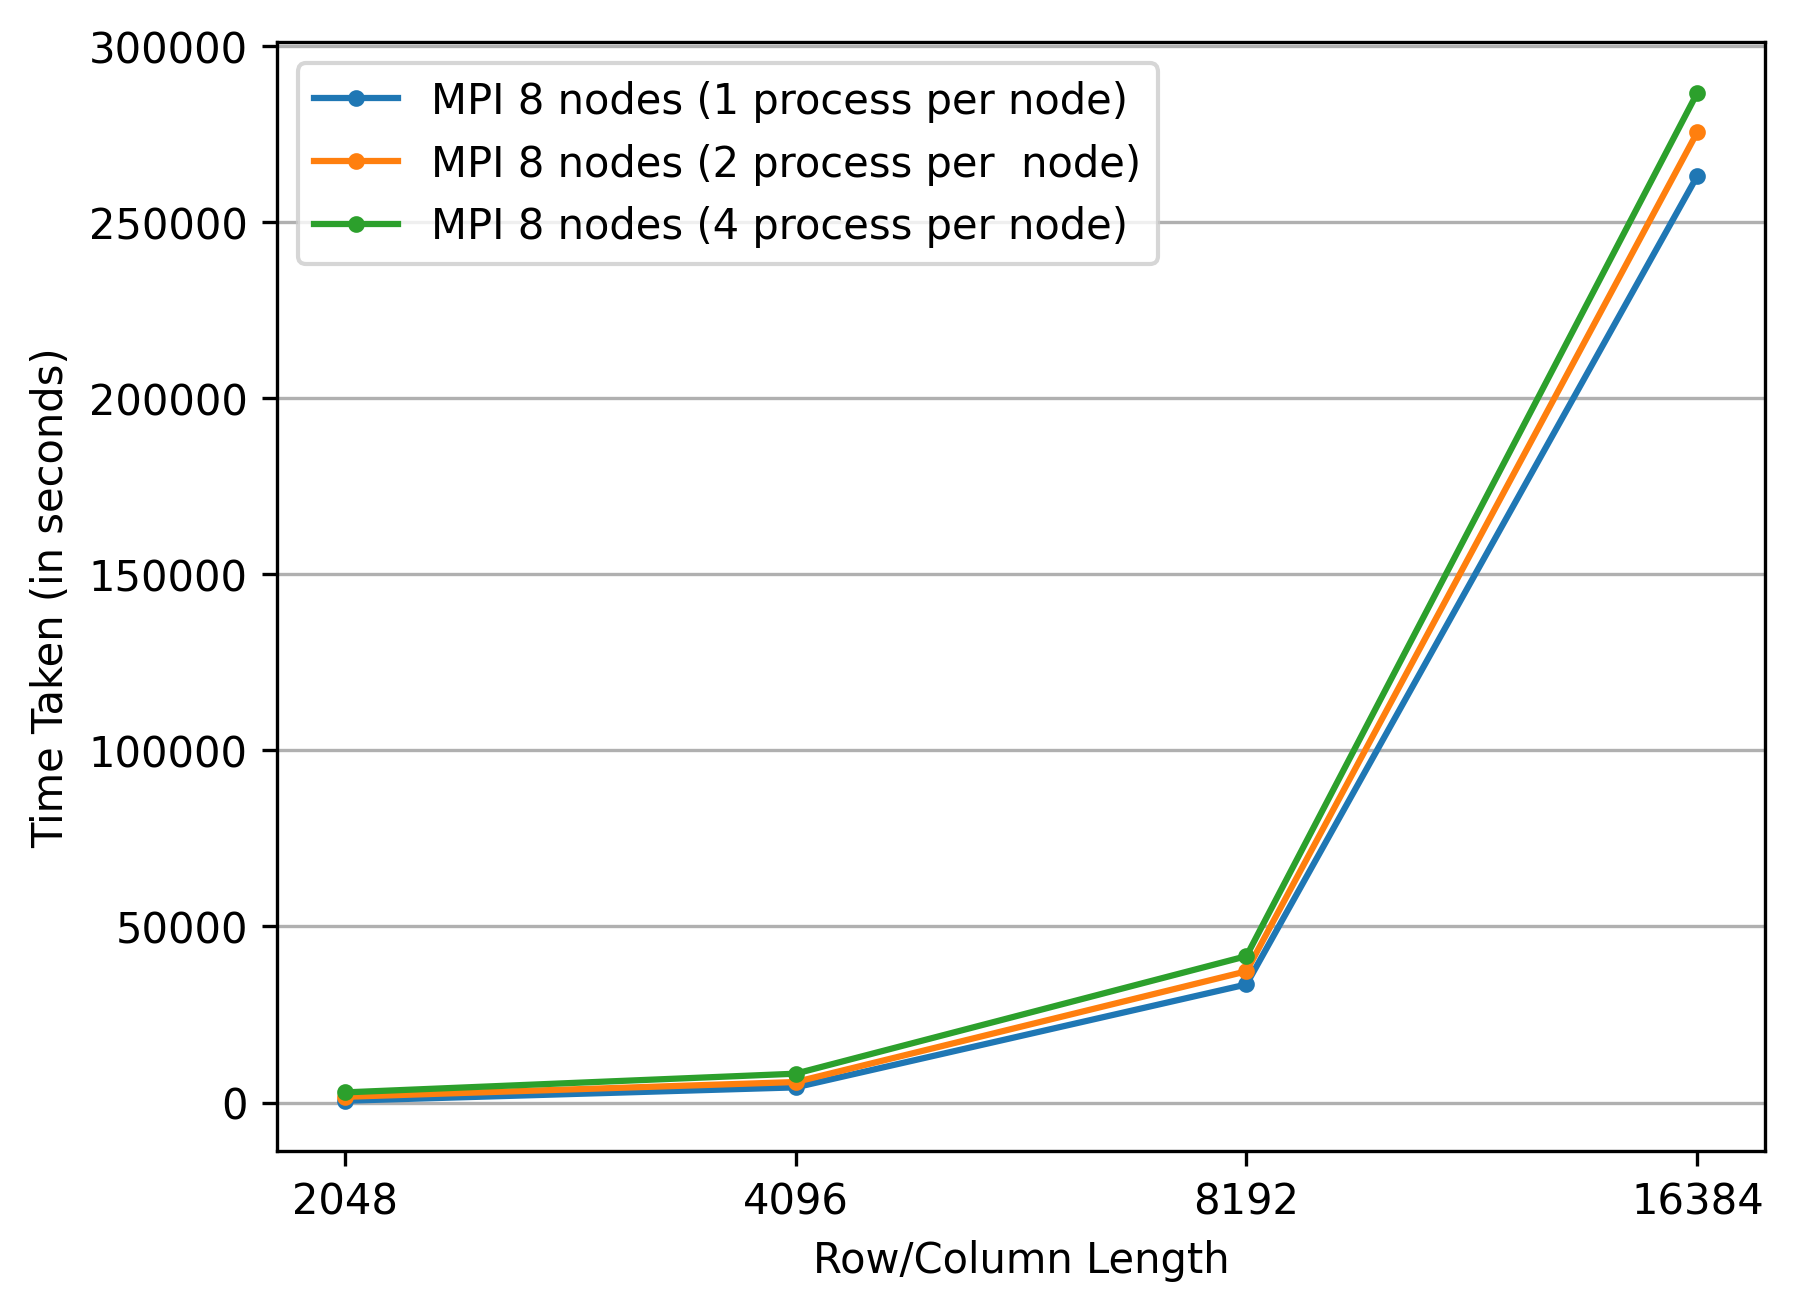
\includegraphics[width=\textwidth]{img/MPI/mpi_threads.png}
        \caption{Comparison giving more threads per node}
        \label{MPI_THEADS}
    \end{minipage}
    
    % First row: Two images adjacent
    \begin{minipage}[t]{0.49\textwidth}
        \centering
        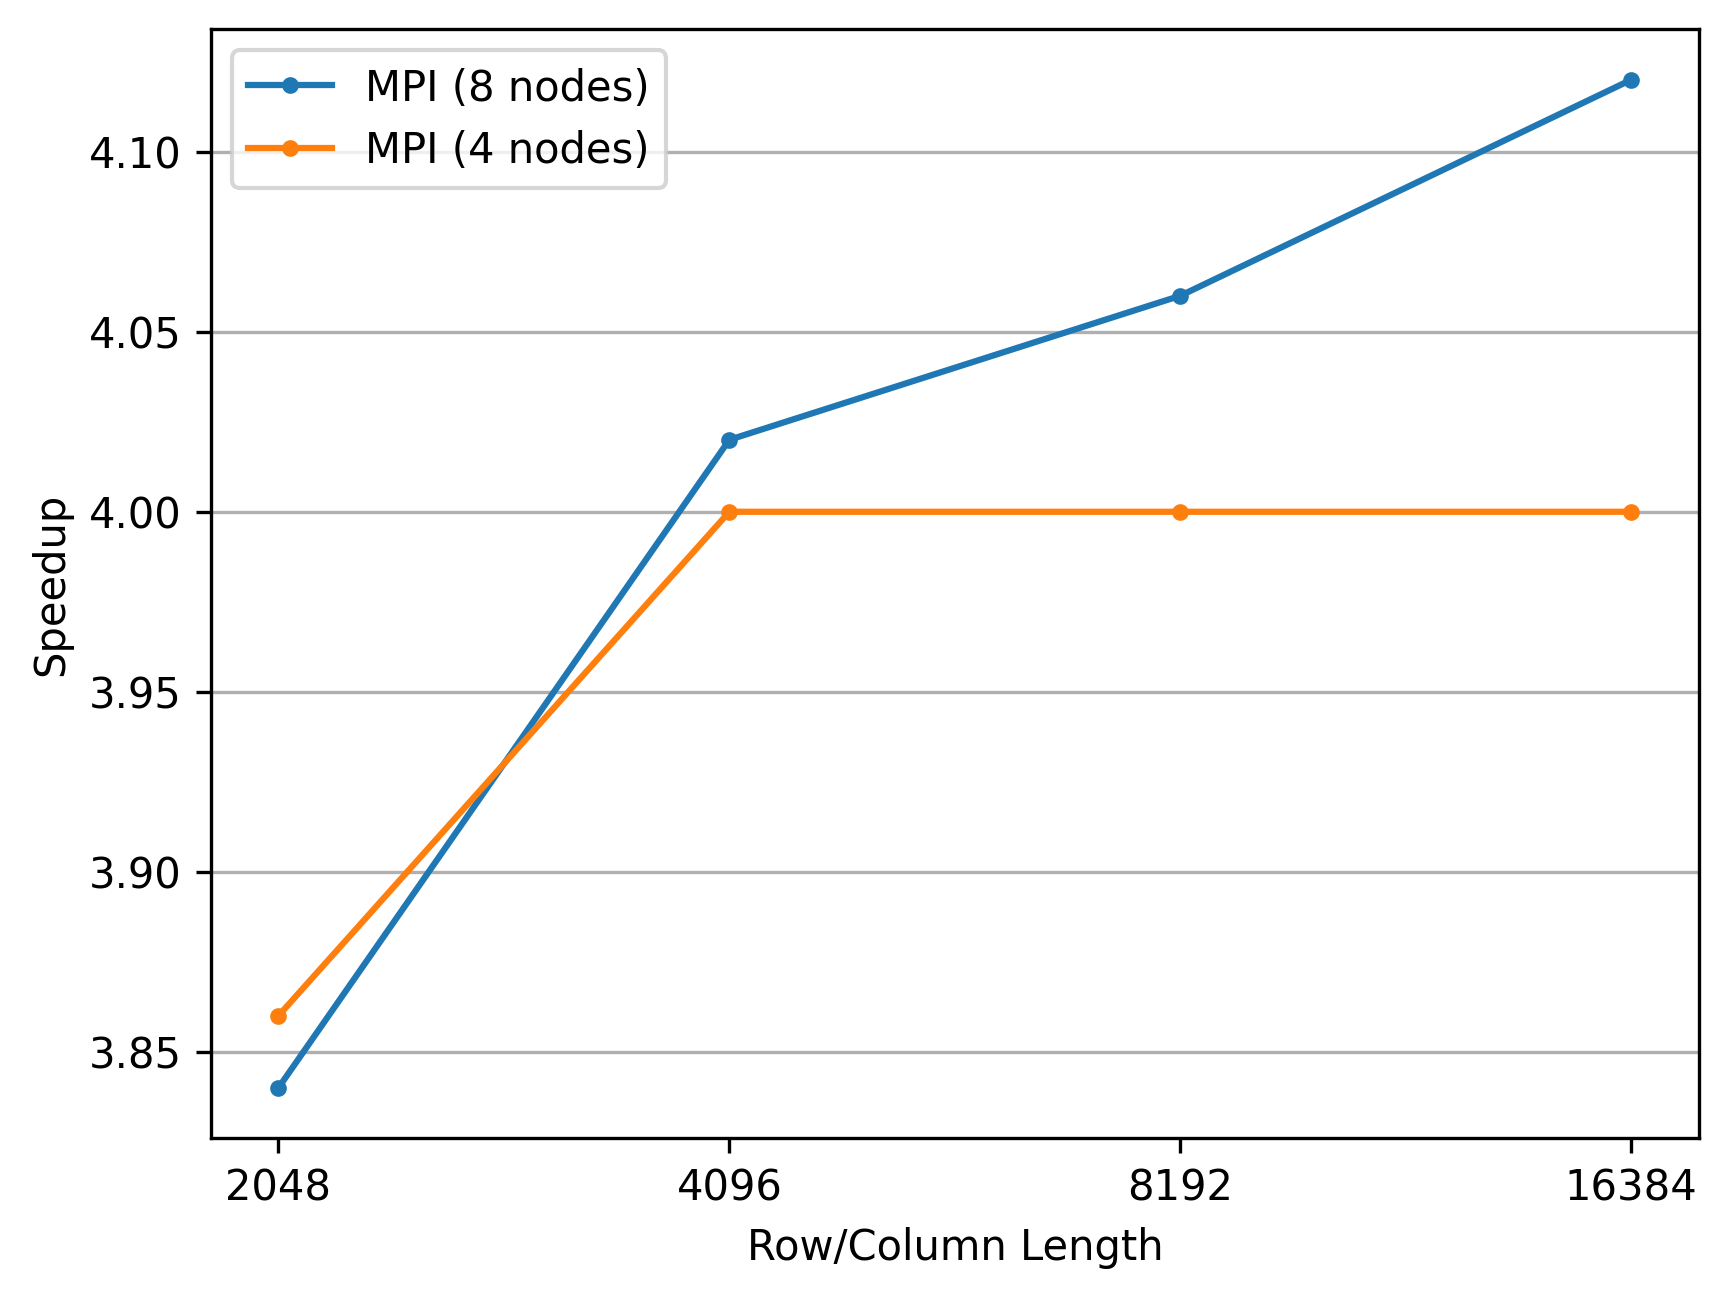
\includegraphics[width=\textwidth]{img/MPI/mpi_speedup.png}
        \caption{Speedup comparison in MPI}
        \label{MPI_Speedup}
    \end{minipage}
    \hfill
    \begin{minipage}[t]{0.49\textwidth}
        \centering
        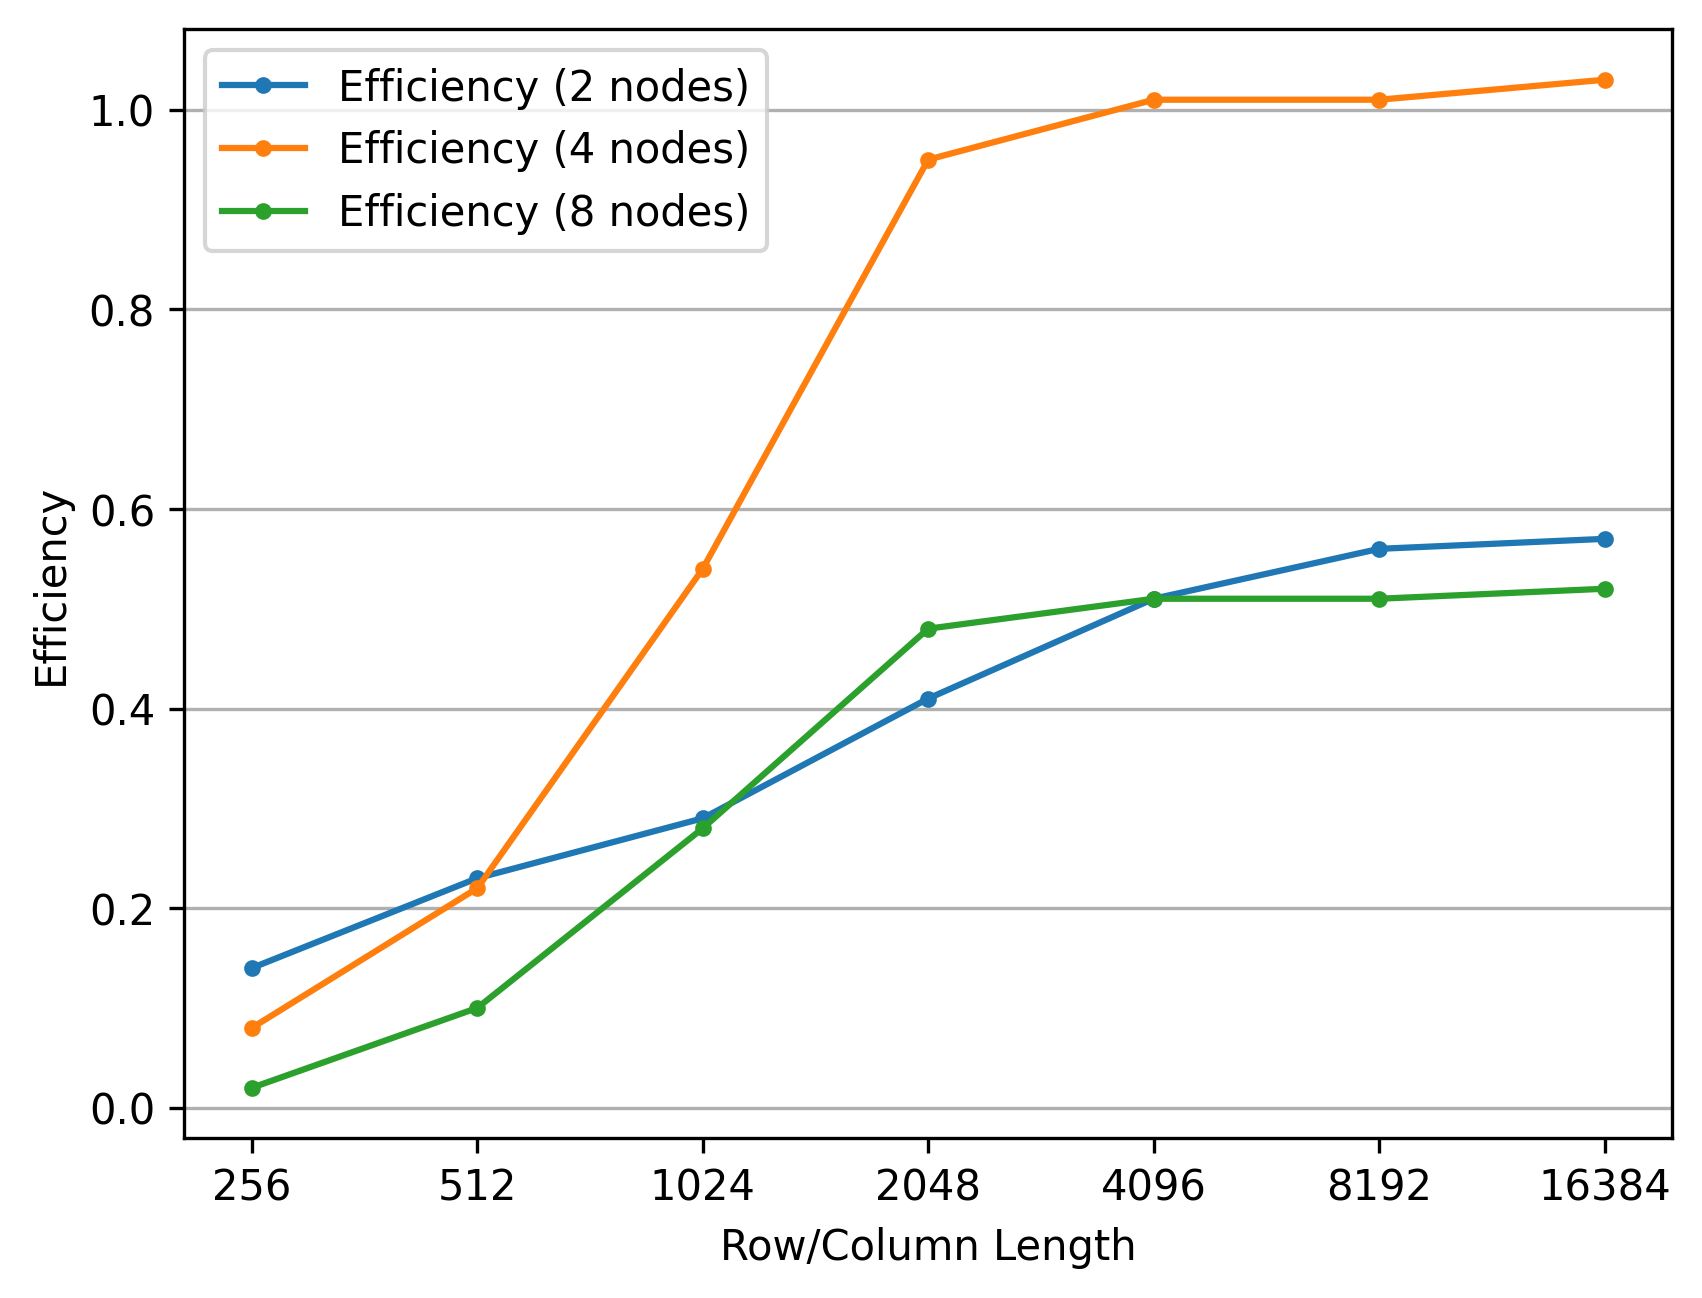
\includegraphics[width=\textwidth]{img/MPI/mpi_efficiency.png}
        \caption{Efficiency comparison in MPI}
        \label{MPI_Efficiency}

    \end{minipage}
    \begin{minipage}[t]{0.90\textwidth}
        \centering
        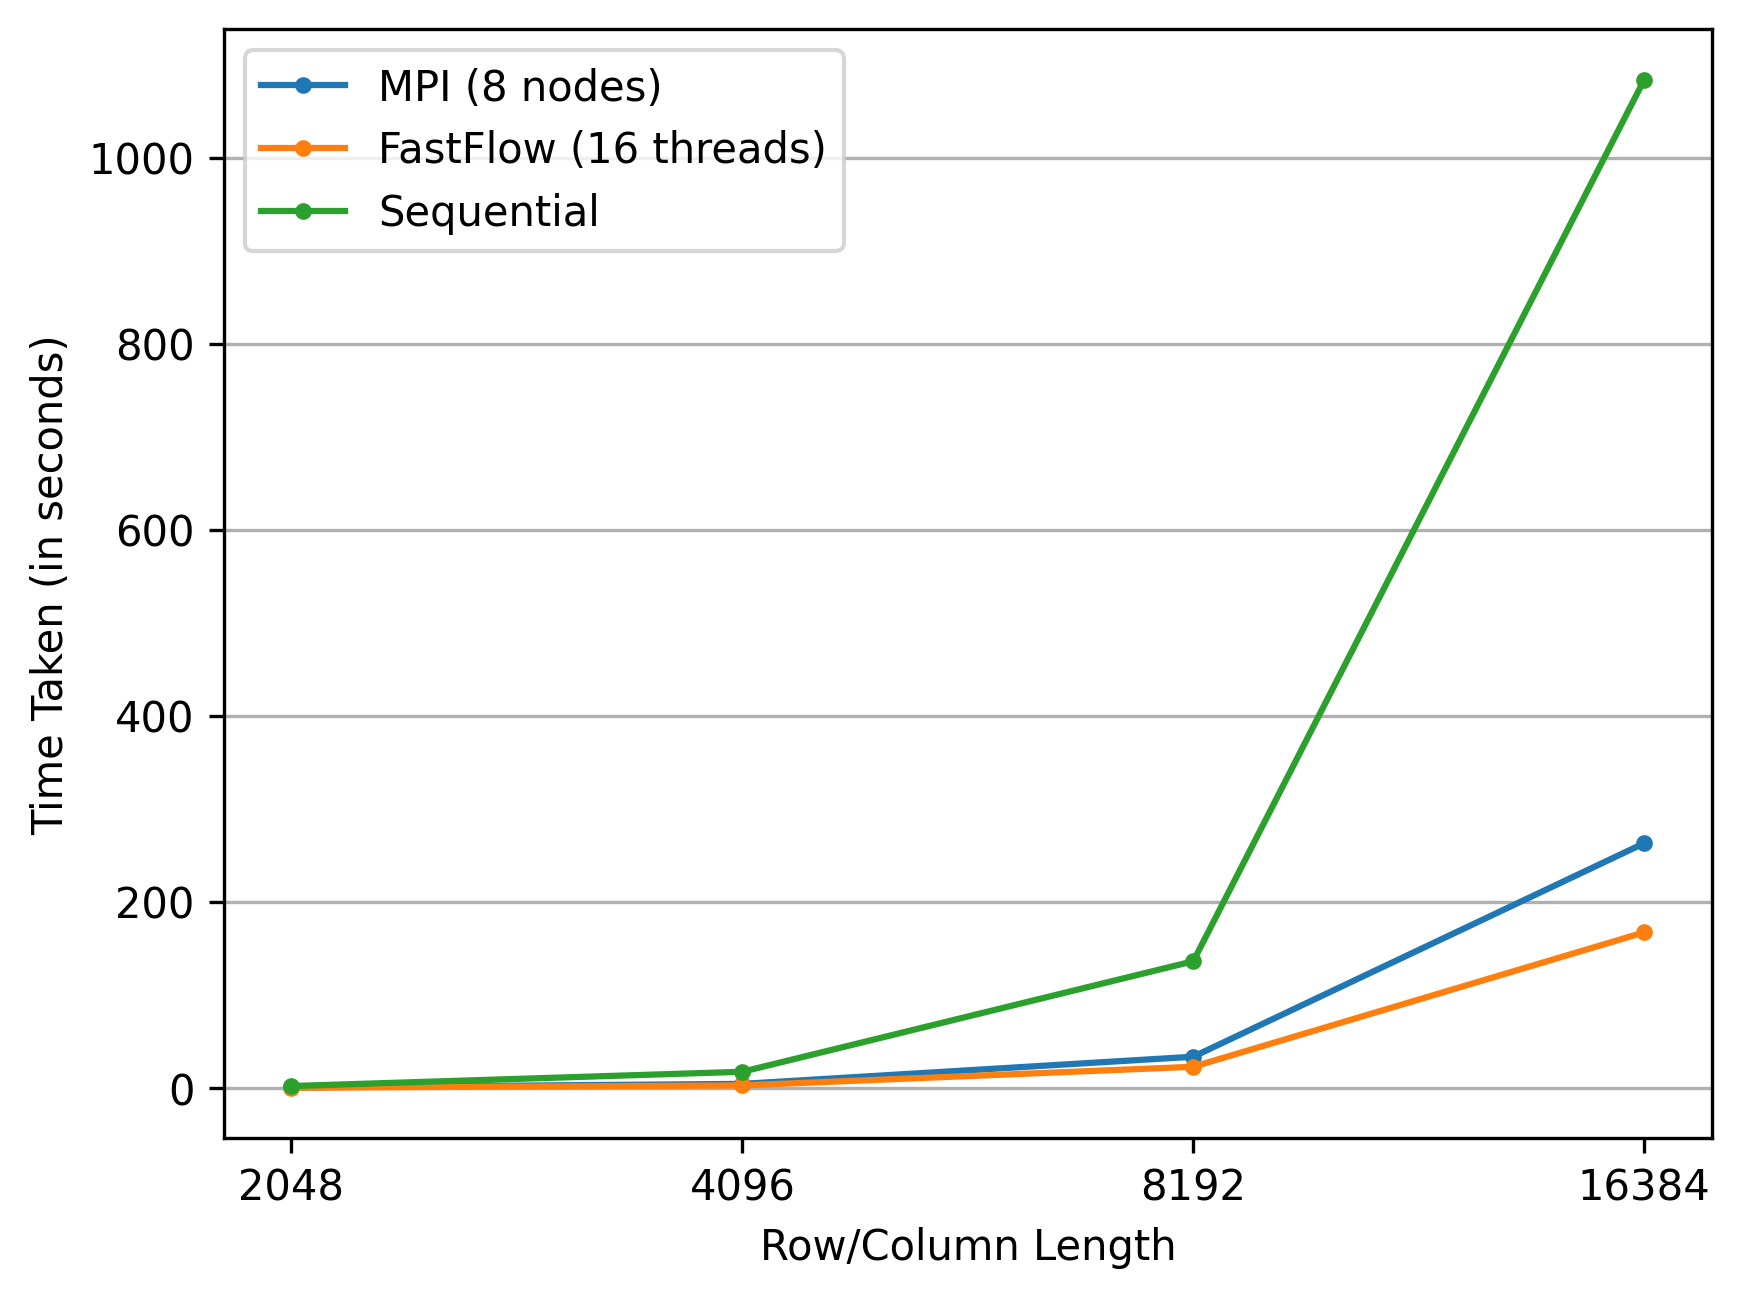
\includegraphics[width=\textwidth]{img/MPI/general_comparison.png}
        \caption{A general comparison between all implementation}
        \label{FF_Chunk}
    \end{minipage}
\end{figure}

\section*{Project Structure}
The project is available on GitHub at the repository: \href{https://github.com/Sallo97/SPM_Project-Wavefront_Pattern}{https://github.com/Sallo97/SPM\_Project-Wavefront\_Pattern}. The root directory includes a CMake file for compiling the project (details provided in the next section), a document describing the project, this report, a README with a brief overview and compilation instructions, and the following folders:

\begin{itemize} 
    \item \textbf{include:} Includes support libraries, specifically the \texttt{FastFlow} library for this project. Before compiling, make sure to run the \textit{``mapping\_string.sh''} script to ensure that \texttt{FastFlow} compiles and optimizes version of the code for the machine used.

    \item \textbf{results:} Stores \texttt{CSV} files containing the average results of each implementation. Each result is organized into subdirectories based on the implementation.

    \item \textbf{scripts:} Contains \texttt{SLURM} scripts used to measure the performance of the implementations in the compute cluster.

    \item \textbf{src:} Contains the source files for the various implementations. Within this directory, the \textit{``utils''} subfolder holds support header files used throughout the project.
\end{itemize}



\subsection*{Compiling and executing the Project}
To compile the entire project, open the terminal at the project's root directory and run the \texttt{cmake} command. It is recommended to keep the build directory separated from the source directory. To do this, use the command \texttt{cmake -B <build\_folder>}, where \texttt{<build\_folder>} is the name of the directory where you want to store the build files. Then, navigate to this build directory and execute \texttt{make} to compile the project. Following these recommendations, the binaries will be stored in the \texttt{src} subfolder. The binaries are the following:
\begin{itemize}
    \item \texttt{sequential [length the matrix]}: execute a sequential implementation of the Wavefront pattern.
    \item \texttt{parallel\_fastflow\_dynamic\_chunk [length of the matrix] [threads to spawn]}: execute the \texttt{FastFlow} implementation of the Wavefront pattern with the given number of threads as node of the Farm. It computes dynamically the chunk size.
    \item \texttt{parallel\_fastflow\_static\_chunk [length of the matrix] [num of threads to spawn]}: execute the \texttt{FastFlow} implementation of the Wavefront pattern with the given number of threads as node of the Farm. It computes dynamically the chunk size.
    \item \texttt{parallel\_mpi [length of the matrix]}: execute the \texttt{MPI} implementation of the Wavefront pattern. Recall that to run the following binary it is needed to call \texttt{mpirun} in the following way: \texttt{mpirun -N [number of nodes to use] ./parallel\_mpi [length of a row of the matrix]}.
\end{itemize}

The \texttt{scripts} folder contains scripts for each implementation, executing them with various matrix lengths (typically from 256 to 16,384) and, where applicable, different numbers of threads or nodes. These scripts were run on the \textit{``spmcluster.unipi.it''} compute cluster to gather the measurements discussed in this report. Each script generates a \texttt{.out} file in the \texttt{results/<implementation>} directory, recording the time for each execution. The average results of the tests done are saved in \texttt{CSV} files in the results folder. 

\section*{Conclusions}
In this report, I explored two distinct approaches to parallelizing the Wavefront pattern: a shared memory solution using the \texttt{FastFlow} library and a distributed memory approach with \texttt{MPI}. Each implementation comes with its own set of advantages and disadvantages, highlighting the fundamental differences in addressing the problem across different architectures. The analysis revealed that the optimal approach depends on the problem's scale. For small matrices (up to 256), a sequential approach is most efficient. As matrix sizes increase, a shared memory solution like \texttt{FastFlow} becomes more effective. However, the matrices we tested are still relatively small and can be comfortably stored within the memory limits of a single process. For much larger matrices, such as those encountered in data centers, a distributed memory approach like \texttt{MPI} becomes essential. The key takeaway is to always record and compare performance measurements to account for overheads, enabling more effective and efficient parallelization strategies.